%
% File naacl2019.tex
%
%% Based on the style files for ACL 2018 and NAACL 2018, which were
%% Based on the style files for ACL-2015, with some improvements
%%  taken from the NAACL-2016 style
%% Based on the style files for ACL-2014, which were, in turn,
%% based on ACL-2013, ACL-2012, ACL-2011, ACL-2010, ACL-IJCNLP-2009,
%% EACL-2009, IJCNLP-2008...
%% Based on the style files for EACL 2006 by 
%%e.agirre@ehu.es or Sergi.Balari@uab.es
%% and that of ACL 08 by Joakim Nivre and Noah Smith

\documentclass[11pt,a4paper]{article}
\usepackage[hyperref]{naaclhlt2019}
\usepackage{times}
\usepackage{amsmath,amsthm,amsfonts,amssymb,amscd}
\usepackage{latexsym}
\usepackage{graphicx}
\usepackage{multirow}
\usepackage{url}
\usepackage{float} 
\usepackage{tabularx}
\newtheorem{lemma}{Lemma}[section]
\newtheorem{theorem}{Theorem}[section]
\newtheorem{proposition}{Proposition}[section]
\newtheorem{definition}{Definition}[section]
\DeclareMathOperator*{\argmax}{argmax}
\DeclareMathOperator*{\argmin}{argmin}
%\aclfinalcopy % Uncomment this line for the final submission
%\def\aclpaperid{***} %  Enter the acl Paper ID here

%\setlength\titlebox{5cm}
% You can expand the titlebox if you need extra space
% to show all the authors. Please do not make the titlebox
% smaller than 5cm (the original size); we will check this
% in the camera-ready version and ask you to change it back.

\title{Sparse Word Embedding for Multi-domain Machine Translation}

\author{Minh Quang Pham\\
  Affiliation / Address line 1 \\
  Affiliation / Address line 2 \\
  Affiliation / Address line 3 \\
  {\tt email@domain} \\\And
  Second Author \\
  Affiliation / Address line 1 \\
  Affiliation / Address line 2 \\
  Affiliation / Address line 3 \\
  {\tt email@domain} \\}

\date{}

\begin{document}
\maketitle
\begin{abstract}
Finetuning a generic neural machine translation model to a certain domain usually degrade its performance on the other domains, thus it's very difficult to build a unique model which is best for all. Indeed, Catastrophic Forgetting, well-known problem in Machine Learning, states that standard backprogation neural network suffers a lot while there is a shift in training data distribution. However, Finetuning is very costly and unefficient in the industry therefore one best model is always desired. In this paper, we introduce an application of an old technique \cite{P07-1033} in Multi-Domain Neural Machine Translation. By defining general information encoding region and domain-specific encoding region in word embedding vector, we are able to seperate domain-related information flows in forward and backward propagation during training thus to
mitigate the catastrophic interference happens during the training over different domains. Empirically, we achieved a unique model that has comparable score to finetuned models for every domains. Furthermore, our method is simple and could be applied for any architecture.
\end{abstract}

\section{Introduction}
Despite fast developpemnt thanks to new architectures \cite{NIPS2017_7181} \cite{bahdanau2014neural} \cite{D13-1176} \cite{Sutskever2014Sequence}, Machine Translation still struggles with data scarcity. Domain adaptation, or it's special case Multi-domain, is the situation where in-domain data (such as banking) is rare while out-domain data such as news are plenty, one aims to leverage out-domain data to improve quality of Machine Translation system which is perfectible while being trained with only the in-domain dataset. Traditionally, ones train a generic model using a very large corpora then use in-domain dataset to finetune the model. It is ubiquitous that the bias to the in-domain dataset used in finetuning makes model worse in translating other domains, thus that we have not been able to finetune a model to several domains at once. This phenomenon can be implied by well-known problem in Machine Learning, Catastrophic Interference \cite{Michael1989Catastrophic}. When there is a shift in the distribution of training data, standard backpropagation neural network gradually lose information learned from other domains while learning only target domain.\\
In Multi-domain Machine Translation, ones have to deal with polysemies whose meaning can be totally different in different domains, for example, the word "chair" means an household tool in "if you are taking a medicine which may cause low blood pressure when rising from a chair or bed " (extracted from medical corpora EMEA \cite{Tiedemann2009RANLP5}) while the word "chair" means to preside over a meeting in following sentence "The President of the ECB or , in his absence , the Vice-President , chairs the meetings of the Governing Council , the Executive Board and the General Council of the ECB. " (extracted from European Central Bank corpora \cite{Tiedemann2009RANLP5}). Using context information is not sufficient to differ these polysemies. Therefore using the same word embedding for polysemies obstructs the model from differentiating the meaning of a polysemy in one domain from it's other meaning in the other domain. \\
\begin{table}[h]
\resizebox{\columnwidth}{!}{
\begin{tabular}{|l|l|l|}
\hline
English Words & French translation & Domain \\ \hline
security & titre financier & Financial \\
security & s\'ecuti\'e & IT\\
joint & articulaire & medical\\
joint & conjoint & banking\\
chair & chaise & general \\
chair & pr\'esider, pr\'esident & banking \\
\hline
\end{tabular}
}
\caption{Polysemies}
\label{table:polysemy}
\end{table}

\begin{table}[h]
\resizebox{\columnwidth}{!}{\begin{tabularx}{\textwidth}{|| X | X | X | X | X | X | X | X ||}
\hline
English sentence & French translation & Domain \\ 
\hline
"Flu-like" symptoms such as headaches, joint pains, feelings of weakness, dizziness, and tiredness may occur, especially at the start of treatment. & Des symptômes grippaux tels que céphalées, douleurs articulaires, sensation de faiblesse, vertige et asthénie, peuvent survenir, en particulier en début de traitement. & medical \\
\hline
\end{tabularx}
}
\caption{Polysemies}
\label{table:polysemy}
\end{table}
     
In this work, we present a new design for word embedding that is composed of different regions which are activate and deactivate corresponding to domains. To evaluate, we use several test sets representing each domains and two other general test sets.
\section{Related Work}
Multi-domain Machine Translation has largely interested NLP community by its promising applications in industry and its relation to fundamental problems in theory. Researchers have proposed a large range of techniques from Data centric methods to Model centric methods \cite{C18-1111}; \cite{P17-2061}. Data centric methods have goal to collect related-domain data from existing in-domain data by using different techniques such as scoring relatedness by Language Model \cite{P10-2041}; \cite{D11-1033}; \cite{P13-2119} or by metric on the space of sentence embedding \cite{P17-2089} or generating pseudo parallel data \cite{P03-1010}; \cite{C16-1295}; \cite{D14-1023}. On the other hand, Model centric approaches focus on NMT models that are specialized for domain adaptation. The novelty can be either trainining objective; for example \cite{Luong2015SNMT}; \cite{P16-1009}; \cite{D17-1155}; \cite{W17-3205}; \cite{D17-1156}; \cite{C18-1269} or architecture \cite{R17-1049}; \cite{gulcehre2016monolingual}; \cite{W17-4712}, \cite{Biao2017CARENMT}; \cite{N18-2080}; \cite{W18-6313}; \cite{C16-1170}; \cite{P18-2050} or the decoding algorithm \cite{gulcehre2016monolingual}; \cite{I17-2004}. Beside these works, we could also consider "out-of-domain" works such as sequence labeling tasks \cite{P07-1033}; learning multiple visual domains \cite{NIPS2017_6654}. The problem is recently investigated by several interesting works presented in EMNLP 2018 such as \cite{D18-1039}; \cite{D18-1041}. \cite{D18-1041} create in the encoder Domain-specific gate $g^r_i$and Domain-shared gate $g^s_i$ which are generated from domain-specific and domain-shared semantic representations of source sentence $E_r(x)$ and $E_s(x)$ respectively and which select information from units of hidden states $h_i$ by elementwise product $h^r_i = g^r_i \odot h_i$; $h^s_i = g^s_i \odot h_i$. $h^r_i$ and $h^s_i$ will be fed to Domain-specific and Domain-shared attentional mechanisms respectively. While introducing new features in the architecture, \cite{D18-1041} introduces also new objective which is sum of word-level weighted MT objective and objectives of Domain-classifier in source side and target side and Adversarial Domain-classifier in source side. The author have very good approach to well seperate Domain-shared information flow and Domain-specify information flow and determine their contributions to the inference that mitigates the catastrophic interference happens in the network during forward step. 

\section{Proposed method}
\subsection{Problem statement}
\begin{definition}{Domain}
\label{def:1}
Domain is a hypothetical probability that generates a set of corpora. We will denote D(C) is domain of set of corpora C.
\end{definition}

In machine translation, the loss function for training is
\begin{equation}
\begin{split}
E_{(x,y) \sim p_{rel}}[-log(p_{\theta}(y|x))] &= \\
= E_{x \sim p_{rel}(x)}[KL(p_{rel}(y|x) & \mid p_{\theta}(y|x))] + \\
+ E_{x \sim p_{rel}} &[H(p_{rel}(y|x))]
\end{split}
\end{equation}.
Where $p_{\theta}(y|x)) = p(y|x,\theta)$ or $p_{\theta}(y|x)) = p(y,\theta | x)$
 In this quantity, domain is exactly $p_{rel}(x,y)$. However, in the inference or translation, the most important goal is to predict target sentence given source sentence, i.e, to well approximate the conditional probability $p_{rel}(y|x)$. However, this relation could be very different if consider 2 domains generating 2 corpora of different topic. Indeed, in financial document, to translate "security" into "titre financier" is more likely than to translate it into "securit\'e" but in IT document. In reality, to translate correctly with respect to the topic of sentence is very important. We formalize the multi-domain problem for machine translation in following equation
\begin{equation}
\begin{split}
\theta^* = \argmin_{\theta} E_{(x,y) \sim D(C_{i})} [-log & (p_{\theta}(y|x,i))] \; \forall i \in [1..d]
\end{split}
\end{equation}
A trivial solution for this equation is $\theta^* = (\theta^*_{0},...,\theta^*_{d})$ and $p_{(\theta_{0},...,\theta_d)}(y|x,i)$ is independent of $\theta_{j}$ $\forall j \neq i$, i.e, $\exists f:\Omega_i \times C(D_i) \rightarrow [0,1]: f_{\theta_i}(y,x) = p_{(\theta_{0},...,\theta_d)}(y|x,i)$ where $\Omega_i$ is set of all possible values of $\theta_i$. \\
The model above is not different than ensemble of $d$ models specialized for one domain. However, we could mitigate this seperation by using shared paramaters denoted $\theta_s$ then reformulate the model as following: \\
$\theta^* = (\theta^*_{0},...,\theta^*_{d}, \theta_s^*)$ and $p_{(\theta_{0},...,\theta_d, \theta_s)}(y|x,i)$ is independent of $\theta_{j}$ $\forall j \neq i$, i.e, $\exists f:\Omega_i \times \Omega_s \times C(D_i) \rightarrow [0,1]: f_{\theta_i, \theta_s}(y,x) = p_{(\theta_{0},...,\theta_d, \theta_s)}(y|x,i)$ \\ $p_{(\theta_{0},...,\theta_d, \theta_s)}(y|x)$ is independent of $\theta_{j}$ $\forall j$ i.e, $\exists \bar{f}:\Omega_s \times C \rightarrow [0,1]: \bar{f}_{\theta_s}(y,x) = p_{(\theta_{0},...,\theta_d, \theta_s)}(y|x)$
where $\Omega_i$ is set of all possible values of $\theta_i$ and $\Omega_s$ is set of all possible values of $\theta_s$. \\
However, there is a problem that the couple $\theta_s^*$ and $\theta_i^*$ have to be optimal $\forall i \in [1..d]$.\\
Despite the fact that $\theta^* = (\theta^*_{0},...,\theta^*_{d}, \theta_s^*)$ is hardly achieved by backpropagation, we could attempt to optimize $\theta_s$:
\begin{equation}
\theta^*_{s} = \displaystyle{\mathop{\argmin}_{\theta_s}}E_{(x,y) \sim D(\displaystyle{\mathop{\cup}_{i \in [1,..,d]}}C_{i})}[-log(p_{\theta_s}(y|x))]
\end{equation} 
then optimize each $\theta_i$ (as additional factor used for fine-tuning the model to the domain $D(C_{i})$) the perplexity with respect to true distribution of domain
\begin{equation}
\theta^*_{i} = \displaystyle{\mathop{\argmin}_{\theta_i}}E_{(x,y) \sim D(C_{i})}[-log(p_{\theta_i,\theta^*_s}(y|x,i))]
\end{equation} 
Our first approach to multi-domain machine translation is to build such trivial solution in calibrating positions and sizes of domain paramters $\theta_i$ and shared parameters $\theta_s$ inside one architecture.
\subsection{Sparse word embedding}
This section explains a new design for word embedding used in multi-domain model. As mentioned above, we separate parameter set into $D+1$ parameter sets correspond to D domains and one shared paramater set. Our first attempt is to split standard vector word embedding into $D+1$ regions named $\theta_i$ for $i \in [1,..,D]$ and $\theta_s$.
\begin{figure}[h]
\center
    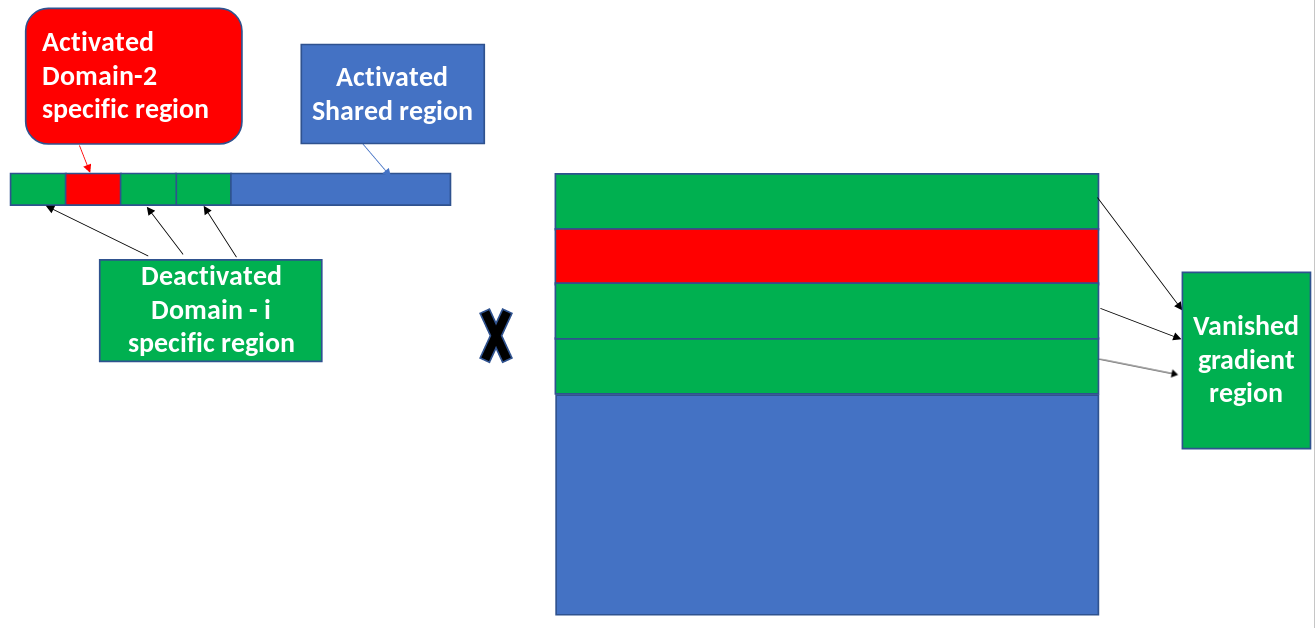
\includegraphics[width=0.8\linewidth]{Sparse1}
    \caption{Sparse word embedding. The red region contains activate units used only when presenting its correpondence domain, the other green regions are deactivate, the bleu generic region is always activate} 
    \label{network}
\end{figure}
The figure \ref{network} presents our proposed design. During backprogation, the rotation matrix receive vanished gradient at regions corresponding to deactivate regions in word embedding. Those regions are also vanished in forward step, thus do not interfere the training on the domain to which they does not correspond.\\
Denote $p_{t} = P * w_{t}$ where $w_{t}$ is word embedding of token $x_{t}$  is projection of word embedding (Transformer \cite{NIPS2017_7181}, Recurrent \cite{bahdanau2014neural})
Assume $x_{t}$ is in domain i, thus, $w_j(t) = 0 \forall j \neq i$. Denote $P_j$ are rows of projection matrix $P$ corresponding to deactivate region $w_j$.
\begin{equation}
\begin{split}
\frac{\partial L(y_t,x_t)}{\partial P_j} &=\frac{\partial L}{\partial p}(p_t) * \frac{\partial p_t}{\partial P_j} \\
								&= \frac{\partial L}{\partial p}(p_t) * w_j(t)\\
									&=0
\end{split} 
\forall j \neq i
\end{equation}
\subsection{Detailed implementation}
The complex structure of State-of-the-art architecture Transformer \cite{NIPS2017_7181} and popular recurrent network \cite{bahdanau2014neural} makes the implementation of sparse embedding non-obvious. Indeed, Transformer involve positional embedding and residual connections which are not homogeneous for domain-regions. Therefore, in our first implementation, we used an dense layer to fuse domain-region and generic region before applying positional embedding and residual connection. This implementation limits the finetuning effect at only word level.\\
Furthermore, because word embeddings are involved in three parts of standard encoder-decoder structure, which are input of encoder, input of decoder and projection before softmax, we have 7 possibilities to apply sparse embedding. However, due to high memory cost, we only want to apply sparse embedding in encoder.
\section{Experiments}
\subsection{Domains and data}
To evaluate the performance of proposed architecture, we use 4 corpora for training: European Medicines Agency; European Central Bank, News-commentary and European Parliament \cite{Tiedemann2009RANLP5} corresponding to 4 domains: medical, banking, news and administrative  respectively and one non-domain corpora Common-crawl  which was introduced in Shared Task: Machine Translation of News the Third Conference On Machine Translation 2018(WMT2018). We use Khresmoi-dev, a test set used in the Biomedical Translation Task (WMT2018), newstest2008, and test2006 as validation set for domains: medical, news administrative; except for banking domain, we use a subset of size 2000 extracted from original corpora and excluded from training set. To test the model, we use Khresmoi-test; newstest2009 and test2007 for domains: medical, news administrative; except for banking domain, we use a subset of size 2000 extracted from original corpora and excluded from training set. The information of used corpora is presented in table \ref{table:Corpora}

\begin{table}[H]
\resizebox{\columnwidth}{!}{
\begin{tabular}{ |l|l|l|l|l|l| }
\hline
Task & Corpora & Train & Dev & Test & Vocabulary \\ \hline
\multirow{5}{*}{$English \rightarrow French$} & European Medicines Agency & 1092568 & 500 & 1000 & \\
 & European Central Bank & 191960 & 2000 & 2000 &\\
 & News-commentary & 258432 & 2051 & 3027 & \\
 & European Parliament & 2007723 & 2000 & 2000 & \\
 & Common-crawl & 3244152 &  &  & \\ \hline
\multirow{5}{*}{$English \rightarrow German$} & European Medicines Agency & 1108752 & 500 & 1000 & \\
 & European Central Bank & 109174 & 2000 & 2000 &\\
 & News-commentary & 270769 & 2051 & 2525 & \\
 & European Parliament & 1920209 & 2000 & 2000 & \\ 
 & Common-crawl & 2399123 &  &  & \\ \hline
\hline
\end{tabular}
}
\caption{Corpora}
\label{table:Corpora}
\end{table}

\subsection{NMT engine}

\subsection{Results}
\begin{figure}[h]
\begin{center}
 \resizebox{\columnwidth}{!}{\begin{tabularx}{\textwidth}{|| X | X | X | X | X | X | X | X ||} 
 \hline
 Models & EMEA test & EPPS test & ECB test & khresmoi (EMEA domain) & test 2007 (EPPS domain) & newstest 2009 & IWSLT 2010 \\ [0.5ex] 
 \hline\hline
 Mixed & 67.69 & 37.5 & 53.49 & 34.86 & 30.96 & 20.98 & 25.7 \\
 \hline
 EMEA-finetuned & 76.77 & 17.16 & 11.99 & 29.58 & 14.25 & 9.92 & 11.10 \\
 \hline
 EPPS-finetuned & & & & & & & \\
 \hline
 ECB-finetuned & & & & & & & \\
 \hline
 Sparse(1) & 70.45 & 38.23 & 54.69 & 34.66 & 31.24 & 21.36 & 26.02 \\
 \hline
 Sparse(2) & 69.91 & 38.05 & 54.2 & 35.22 & 31.25 & 21.36 & 26.02 \\
 \hline
 Sparse(3) &  &  &  &  &  &  & \\
 \hline
 Domain Control & 67.87 & 37.31 & 54.14 & 33.63 & 31.09 & & \\
 \hline
\end{tabularx}}
\end{center}
\caption{bpe-detokenized BLEU score in language pair English - French. Sparse(1) uses correponding domain tag for EMEA, EPPS, ECB test sets and generic tag for newstest and IWSLT. Sparse(2) uses generic tag for all of test sets. Sparse(3) uses tag predicted by pretrained domain classififer}
\label{tab:1}
\end{figure}

\begin{figure}[h]
\caption{BLEU score in language pair English - German}
\begin{center}
 \resizebox{\columnwidth}{!}{\begin{tabularx}{\textwidth}{|| X | X | X | X | X | X | X | X ||} 
 \hline
 Models & EMEA test & EPPS test & ECB test & khresmoi (EMEA domain) & test 2007 (EPPS domain) & newstest 2009 & IWSLT 2010 \\ [0.5ex] 
 \hline\hline
 Mixed & & & & & & & \\
 \hline
 EMEA-finetuned & & & & & & & \\
 \hline
 EPPS-finetuned & & & & & & & \\
 \hline
 ECB-finetuned & & & & & & & \\
 \hline
 Sparse & & & & & & & \\
 \hline
 Domain Control & & & & & & & \\
 \hline
\end{tabularx}}
\end{center}
\label{tab:2}
\end{figure}
\section{Conclusions}

\section*{Acknowledgments}

\bibliography{naaclhlt2019}
\bibliographystyle{plainnat}

\end{document}
